\FloatBarrier
\begin{figure}[!h]
\centering
\subfloat[Zustand in dem im Diodenlaser keine Besetzungsinversion vorliegt und das
	emittierte dem einer LED 
	gleicht. Bei einem Strom $I = \SI{30.0}{\milli\ampere}$ aufgenommen.
	\label{fig:diodenlaser_aus}]{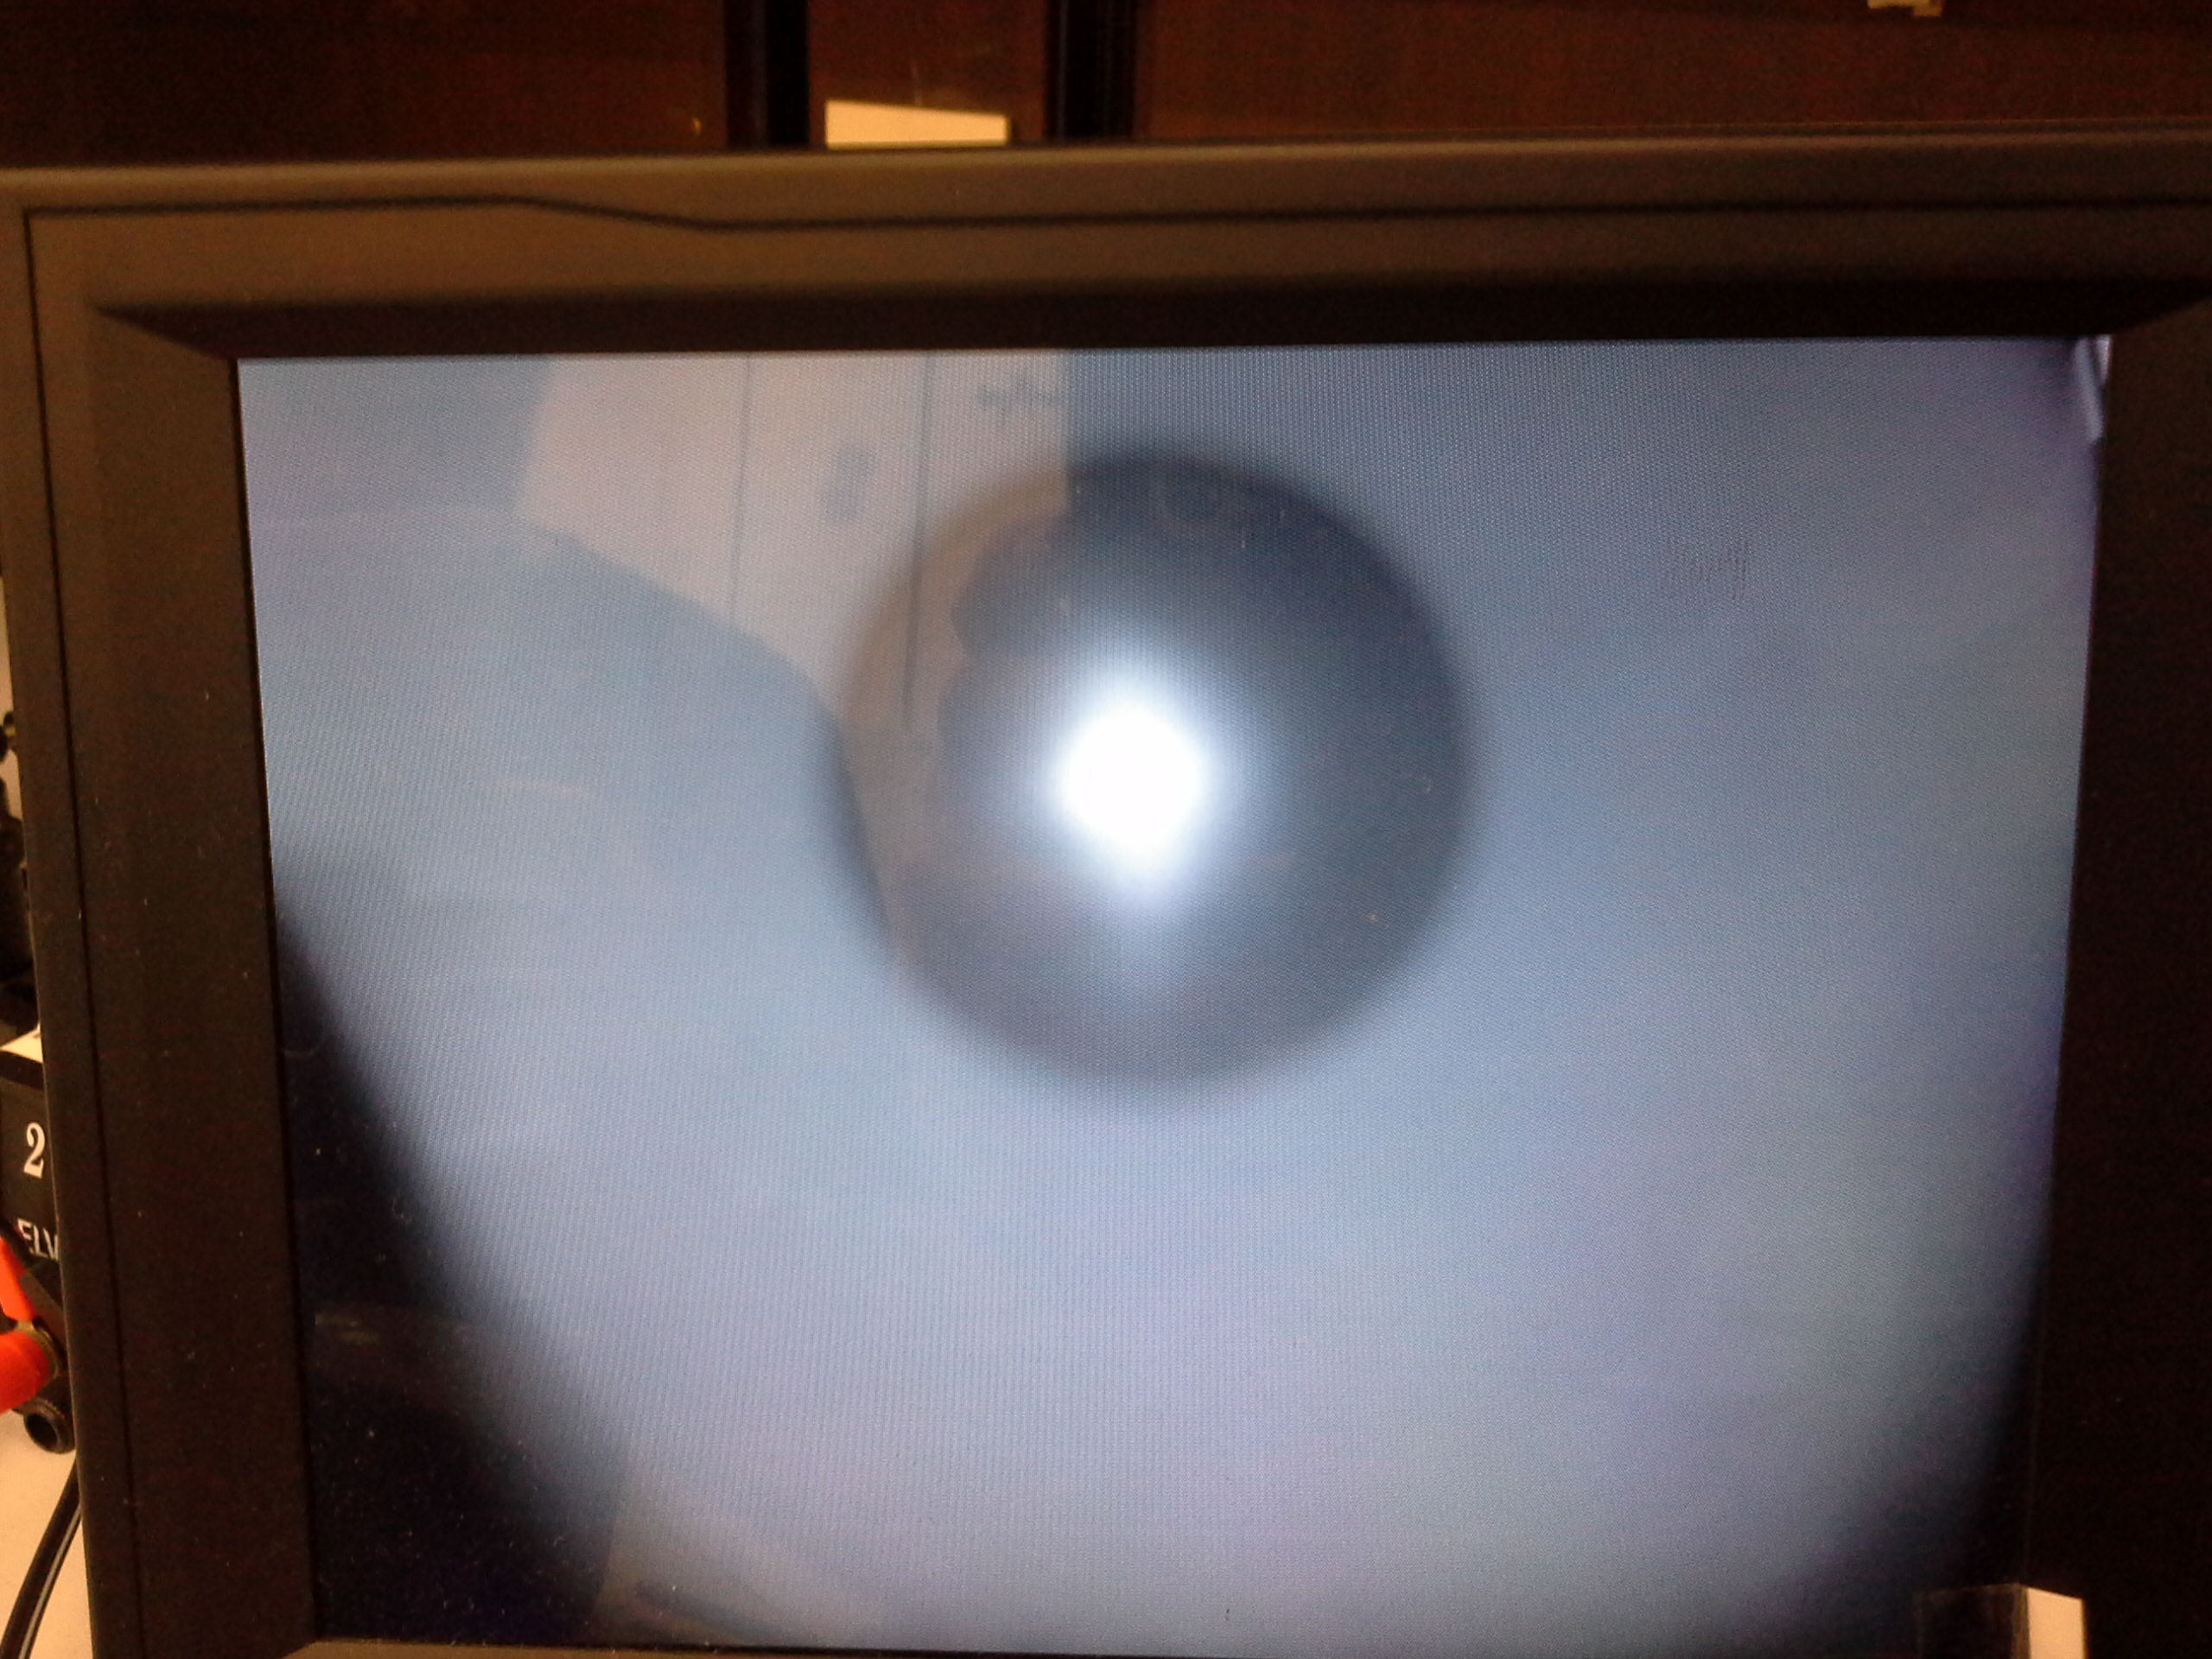
\includegraphics[scale=0.08]{../Grafiken/Diodenlaser_aus.jpg}}
\qquad
\subfloat[Zustand in dem im Diodenlaser Besetzungsinversion vorliegt und dieser zu lasen beginnt.
Das es sich bei dem hier zu beobachtenden Schein um kohärente Licht handelt ist an den einzeln
zu erkennenden Leuchtpunkten (den sogenannten speckles) am Rand des Strahles zu erkennen.
An der geringsten Strom $I = \SI{30.4}{\milli\ampere}$ aufgenommen, bei dem der Laser noch
zum lasen gebracht werden konnte.
\label{fig:diodenlaser_an}]{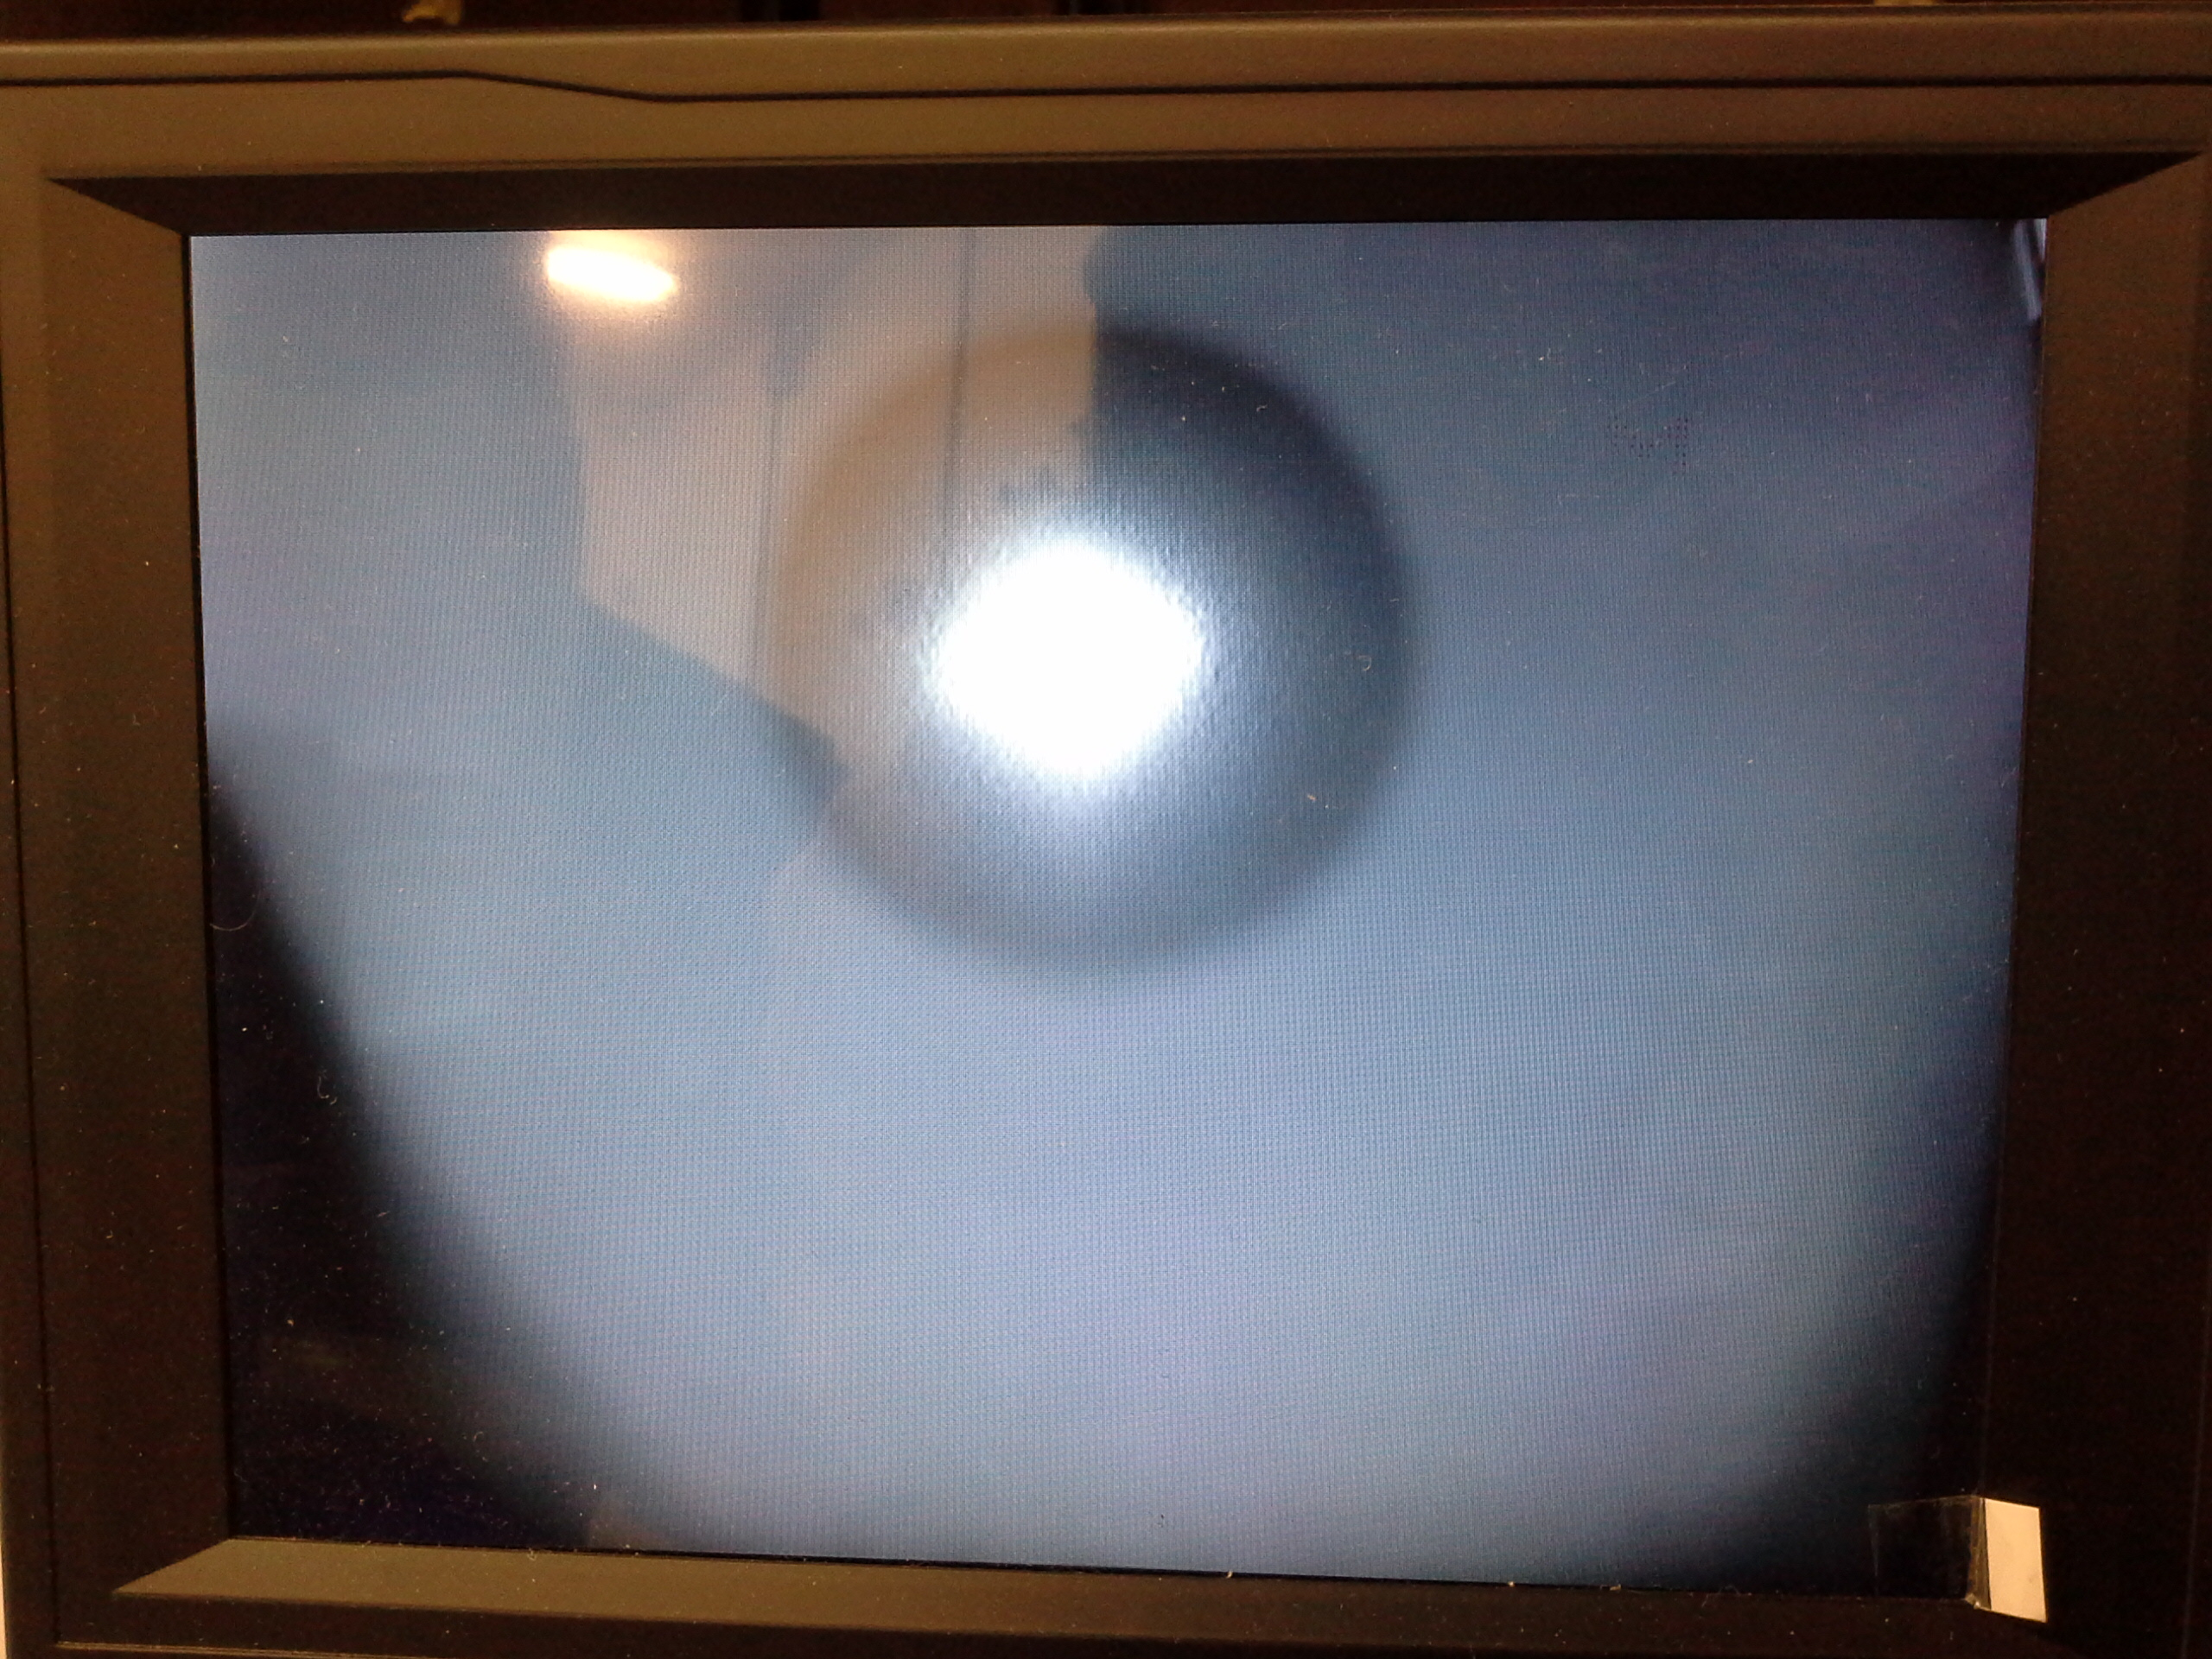
\includegraphics[scale=0.08]{../Grafiken/Diodenlaser_an.jpg}}

\caption{Bilder der beiden unterschiedlichen Emissionsarten des Diodenlasers, durch eine IR-Sichtkarte 
	sichtbar gemacht.\label{fig:diodenlaser_zustand}}
\end{figure}
\FloatBarrier